\documentclass[tikz,border=15pt]{standalone}
\usepackage{tikz}
\usepackage{xcolor}
\usetikzlibrary{shapes.geometric,calc}

\definecolor{bgcream}{RGB}{255,248,240}
\definecolor{furcolor}{RGB}{186,122,72}
\definecolor{furdark}{RGB}{140,85,45}
\definecolor{innercolor}{RGB}{244,210,184}
\definecolor{snoutcolor}{RGB}{255,235,214}
\definecolor{stitchcolor}{RGB}{122,69,34}
\definecolor{patchcolor}{RGB}{252,241,217}
\definecolor{patchborder}{RGB}{214,124,124}
\definecolor{patchstitch}{RGB}{179,84,84}
\definecolor{bowcolor}{RGB}{200,62,62}
\definecolor{bowdark}{RGB}{142,32,32}
\definecolor{shadowdark}{RGB}{66,37,16}
\definecolor{shadowlight}{RGB}{107,68,38}
\definecolor{cheekpink}{RGB}{240,136,120}
\definecolor{nosebrown}{RGB}{69,38,19}
\definecolor{eyeblack}{RGB}{26,14,7}

\begin{document}
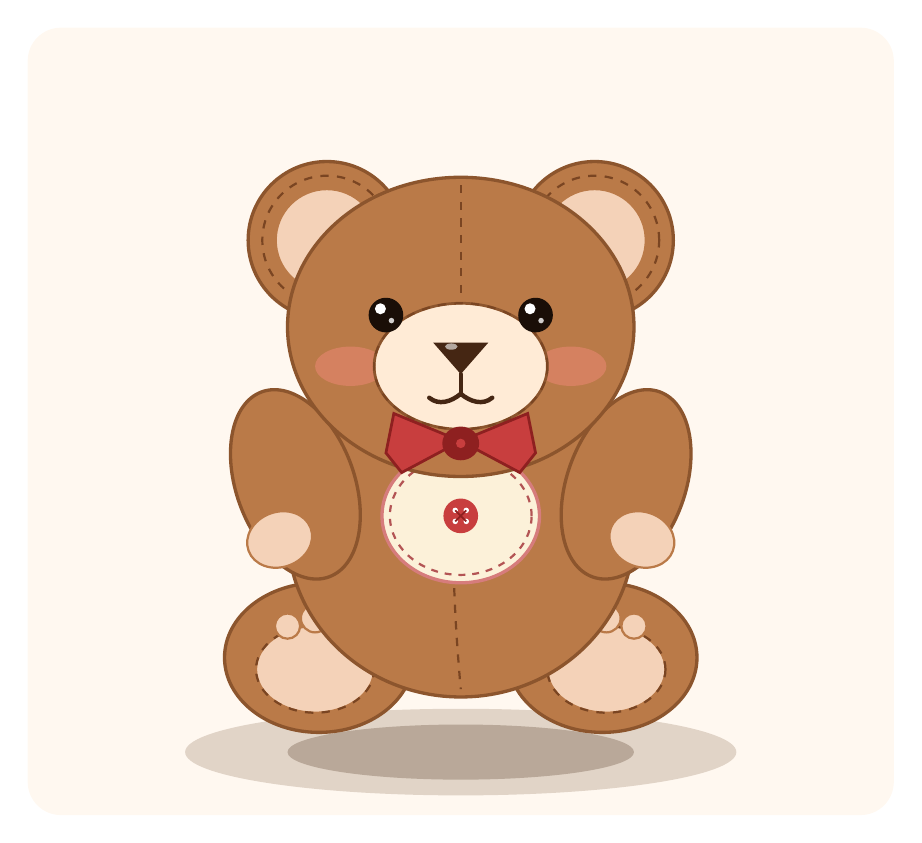
\begin{tikzpicture}[
    fur/.style={fill=furcolor, draw=furdark, line width=1.2pt},
    innerfur/.style={fill=innercolor, draw=furcolor, line width=0.8pt},
    snout/.style={fill=snoutcolor, draw=furdark, line width=1pt},
    stitch/.style={draw=stitchcolor, dashed, dash pattern=on 3pt off 3pt, line width=0.8pt},
    patch/.style={fill=patchcolor, draw=patchborder, line width=1.2pt},
    patchst/.style={draw=patchstitch, dashed, dash pattern=on 2.5pt off 2.5pt, line width=0.8pt},
    bowtie/.style={fill=bowcolor, draw=bowdark, line width=1pt}
]

% Background Soft Warm Box
\fill[rounded corners=12pt, fill=bgcream] (-5.5,-4.8) rectangle (5.5,5.2);

% Floor Shadow
\fill[fill=shadowlight, opacity=0.2] (0,-4.0) ellipse (3.5cm and 0.55cm);
\fill[fill=shadowdark, opacity=0.25] (0,-4.0) ellipse (2.2cm and 0.35cm);

% 1. EARS
\fill[fur] (-1.7, 2.5) circle (1.0cm);
\fill[innerfur] (-1.7, 2.5) circle (0.65cm);
\draw[stitch] (-1.7, 2.5) circle (0.82cm);

\fill[fur] (1.7, 2.5) circle (1.0cm);
\fill[innerfur] (1.7, 2.5) circle (0.65cm);
\draw[stitch] (1.7, 2.5) circle (0.82cm);

% 2. LEGS & FEET (sitting pose)
\fill[fur] (-1.8, -2.8) ellipse (1.2cm and 0.95cm);
\fill[innerfur] (-1.85, -2.95) ellipse (0.75cm and 0.55cm);
\draw[stitch] (-1.85, -2.95) ellipse (0.75cm and 0.55cm);
\fill[innerfur] (-2.2, -2.4) circle (0.16cm);
\fill[innerfur] (-1.85, -2.3) circle (0.18cm);
\fill[innerfur] (-1.5, -2.4) circle (0.16cm);

\fill[fur] (1.8, -2.8) ellipse (1.2cm and 0.95cm);
\fill[innerfur] (1.85, -2.95) ellipse (0.75cm and 0.55cm);
\draw[stitch] (1.85, -2.95) ellipse (0.75cm and 0.55cm);
\fill[innerfur] (1.5, -2.4) circle (0.16cm);
\fill[innerfur] (1.85, -2.3) circle (0.18cm);
\fill[innerfur] (2.2, -2.4) circle (0.16cm);

% 3. BODY
\fill[fur] (0, -1.2) ellipse (2.2cm and 2.1cm);
\draw[stitch] (0, 0.4) to[out=-95, in=95] (0, -3.2);

% Tummy Patch
\fill[patch] (0, -1.0) ellipse (1.0cm and 0.85cm);
\draw[patchst] (0, -1.0) ellipse (0.9cm and 0.75cm);

% Heart / Button on Patch
\fill[fill=bowcolor] (0, -1.0) circle (0.22cm);
\fill[white] (-0.07, -0.93) circle (0.035cm);
\fill[white] (0.07, -0.93) circle (0.035cm);
\fill[white] (-0.07, -1.07) circle (0.035cm);
\fill[white] (0.07, -1.07) circle (0.035cm);
\draw[draw=bowdark, line width=0.6pt] (-0.07, -0.93) -- (0.07, -1.07);
\draw[draw=bowdark, line width=0.6pt] (-0.07, -1.07) -- (0.07, -0.93);

% 4. ARMS
\fill[fur, rotate around={20:(-2.1, -0.6)}] (-2.1, -0.6) ellipse (0.75cm and 1.25cm);
\fill[innerfur, rotate around={20:(-2.3, -1.3)}] (-2.3, -1.3) ellipse (0.42cm and 0.35cm);

\fill[fur, rotate around={-20:(2.1, -0.6)}] (2.1, -0.6) ellipse (0.75cm and 1.25cm);
\fill[innerfur, rotate around={-20:(2.3, -1.3)}] (2.3, -1.3) ellipse (0.42cm and 0.35cm);

% 5. HEAD
\fill[fur] (0, 1.4) ellipse (2.2cm and 1.9cm);
\draw[stitch] (0, 3.2) -- (0, 1.8);

% Cheeks
\fill[cheekpink, opacity=0.5] (-1.4, 0.9) ellipse (0.45cm and 0.25cm);
\fill[cheekpink, opacity=0.5] (1.4, 0.9) ellipse (0.45cm and 0.25cm);

% 6. SNOUT
\fill[snout] (0, 0.9) ellipse (1.1cm and 0.8cm);
\draw[stitch] (0, 0.9) ellipse (1.1cm and 0.8cm);

% Nose
\fill[nosebrown] (-0.35, 1.2) -- (0.35, 1.2) -- (0, 0.8) -- cycle;
\fill[white, opacity=0.6] (-0.12, 1.15) ellipse (0.08cm and 0.04cm);

% Mouth
\draw[nosebrown, line width=1.6pt, line cap=round] (0, 0.8) -- (0, 0.55);
\draw[nosebrown, line width=1.6pt, line cap=round] (-0.4, 0.5) to[out=-40, in=-140] (0, 0.55) to[out=-40, in=-140] (0.4, 0.5);

% 7. EYES
\fill[eyeblack] (-0.95, 1.55) circle (0.22cm);
\fill[white] (-1.02, 1.63) circle (0.07cm);
\fill[white, opacity=0.8] (-0.88, 1.48) circle (0.035cm);

\fill[eyeblack] (0.95, 1.55) circle (0.22cm);
\fill[white] (0.88, 1.63) circle (0.07cm);
\fill[white, opacity=0.8] (1.02, 1.48) circle (0.035cm);

% 8. BOW TIE
\fill[bowtie] (0, -0.05) -- (-0.85, 0.3) -- (-0.95, -0.2) -- (-0.75, -0.45) -- cycle;
\fill[bowtie] (0, -0.05) -- (0.85, 0.3) -- (0.95, -0.2) -- (0.75, -0.45) -- cycle;
\fill[fill=bowdark, draw=bowdark, line width=0.8pt] (0, -0.08) ellipse (0.22cm and 0.2cm);
\fill[fill=bowcolor] (0, -0.08) circle (0.06cm);

\end{tikzpicture}
\end{document}
